\chapter{哈密顿力学}\label{ch:b3:hamiltonian-mechanics}

对一个单摆拍摄一千次，
每次都将其角度对角动量作图：这些点落在一条闭合曲线上，
单摆的每一种可能运动都是这样的一条曲线——小幅摆动对应
嵌套的卵形线，整圈转动对应上下两侧的波状曲线，
两者之间是一条将两类运动分隔开来的交叉曲线。
这幅图，即\emph{\omterm{def:b3:hamiltonian-mechanics:portrait}{相图}}，是哈密顿于 1833 年对力学进行重新表述的核心：
系统的状态是坐标\emph{与}动量所构成空间中的一个点，
其演化是该空间中的一条流，
这条流由单一函数——能量——生成，
通过两个形式十分对称的一阶方程。
其收获并不在于计算更简便（这方面通常是拉格朗日占优），
而在于得到正确的\emph{几何}图像：该流保持\omterm{def:b3:hamiltonian-mechanics:hamiltonian}{相空间}体积不变，
这一性质将奠定统计物理的基础；
其代数骨架，即\omterm{def:b3:hamiltonian-mechanics:poisson}{泊松括号}，恰好是量子力学将要
推广为对易子。本章是连接物体力学与
二十世纪物理学的枢纽。

\section{从拉格朗日到哈密顿}

\begin{definition}[哈密顿量与正则方程]\label{def:b3:hamiltonian-mechanics:hamiltonian}
\index{哈密顿量}\index{正则方程}\index{相空间}
对\omterm{def:b3:lagrangian-mechanics:action}{拉格朗日量}为 $L(q, \dot q, t)$ 的系统，
将速度以动量 $p_i = \partial L/\partial\dot q_i$ 表示，并定义
\emph{哈密顿量}为勒让德变换
\[
H(q, p, t) = \sum_i p_i\dot q_i - L ,
\]
它是坐标与\emph{动量}的函数。
$2n$ 维空间即 $(q_1, \dots, q_n, p_1, \dots, p_n)$ 所构成的空间，
\emph{相空间}；其中的一点，即一个\emph{状态}，
由此确定系统的全部过去与未来，
借助\emph{正则方程}
（见\cref{thm:b3:hamiltonian-mechanics:canonical}）。
\end{definition}

\begin{theorem}[正则方程]\label{thm:b3:hamiltonian-mechanics:canonical}
\omterm{thm:b3:lagrangian-mechanics:euler-lagrange}{欧拉–拉格朗日方程}等价于 $2n$ 个一阶
方程：
\[
\dot q_i = \frac{\partial H}{\partial p_i} , \qquad
\dot p_i = -\frac{\partial H}{\partial q_i} .
\]
\end{theorem}

\begin{proof}
将 $H = \sum p_i\dot q_i - L$ 视为 $(q, p, t)$ 的函数并求微分：
$\dd H = \sum(\dot q_i\,\dd p_i + p_i\,\dd\dot q_i) - \sum(
\partial_{q_i}L\,\dd q_i + \partial_{\dot q_i}L\,\dd\dot q_i) -
\partial_tL\,\dd t$。$\dd\dot q_i$ 项由
$p_i$ 的定义相消——这正是勒让德变换的关键——于是只剩
$\dd H = \sum(\dot q_i\,\dd p_i - \partial_{q_i}L\,\dd q_i) -
\partial_tL\,\dd t$。由偏导数直接读出：
$\partial H/\partial p_i = \dot q_i$ 与 $\partial H/\partial q_i =
-\partial L/\partial q_i$，由\omterm{thm:b3:lagrangian-mechanics:euler-lagrange}{欧拉–拉格朗日方程}，它等于 $-\dot p_i$。
（此外 $\partial_tH = -\partial_tL$。）
\end{proof}

\begin{proposition}[$H$ 的意义]\label{prop:b3:hamiltonian-mechanics:energy}
$H$ 与上一章中的\omterm{prop:b3:lagrangian-mechanics:energy}{能量函数} $h$ 一致：
沿任一运动有 $\dd H/\dd t = \partial H/\partial t$，故 $H$
只要其不显含时间即守恒；当
动能为速度的二次函数、约束与时间无关时，
$H = E_k + E_p$，即机械能，
只是改用变量 $(q, p)$ 表示。
\end{proposition}

\begin{proof}
$\dd H/\dd t = \sum(\partial_{q_i}H\,\dot q_i + \partial_{p_i}H\,\dot
p_i) + \partial_tH = \sum(\partial_{q_i}H\,\partial_{p_i}H -
\partial_{p_i}H\,\partial_{q_i}H) + \partial_tH = \partial_tH$：
\omterm{def:b3:hamiltonian-mechanics:hamiltonian}{正则方程}的对称性使求和项恒等相消。
与 $E_k + E_p$ 的等同
由\cref{prop:b3:lagrangian-mechanics:energy}可知。
\end{proof}

\begin{example}[两个哈密顿量]\label{ex:b3:hamiltonian-mechanics:examples}
弹簧上的质点：$p = m\dot x$，于是
\[
H = \frac{p^2}{2m} + \frac12 kx^2 ;
\]
\omterm{def:b3:hamiltonian-mechanics:hamiltonian}{正则方程} $\dot x = p/m$、$\dot p = -kx$ 即为熟悉的
这一对方程。单摆：$p = m\ell^2\dot\theta$，其\omterm{def:b3:hamiltonian-mechanics:hamiltonian}{哈密顿量}为
\[
H = \frac{p^2}{2m\ell^2} - mg\ell\cos\theta .
\]
两种情形中 $H$ 都是能量，在每一运动中保持常数：
运动\emph{即}为 $H$ 在 $(q,p)$ 平面中的等值线。
\end{example}

\begin{method}[哈密顿方法]\label{met:b3:hamiltonian-mechanics:recipe}
（1）由 $L$ 求出动量 $p_i = \partial L/\partial\dot q_i$，
并解出 $\dot q_i$。（2）写出 $H = \sum p_i\dot q_i - L$，
仅用 $(q, p)$ 表示——对自然系统而言，即 $E_k + E_p$，
其中 $E_k$ 改用动量表示。（3）写出
\omterm{def:b3:hamiltonian-mechanics:hamiltonian}{正则方程}。（4）作出 $H$ 的等值线：对于一个\omterm{def:b3:lagrangian-mechanics:coordinates}{自由度}，
它们即为轨迹，整个定性运动
——振动、转动、平衡态、\omterm{def:b3:hamiltonian-mechanics:portrait}{分界线}——均可直接读出，
无需求解任何方程。
\end{method}

\section{相空间}

\begin{definition}[相图、不动点与分界线]\label{def:b3:hamiltonian-mechanics:portrait}
\index{相图}\index{不动点}\index{分界线}
系统的\emph{相图}是其在\omterm{def:b3:hamiltonian-mechanics:hamiltonian}{相空间}中的
轨迹族。\emph{不动点}是指这样一种状态：
两个\omterm{def:b3:hamiltonian-mechanics:hamiltonian}{正则方程}同时为零——即平衡态：势能的
极小值表现为被闭合曲线环绕的\emph{中心}，极大值
表现为\emph{鞍点}，穿过它的是一条\emph{分界线}，
即这样一条轨迹：它把\omterm{def:b3:hamiltonian-mechanics:hamiltonian}{相空间}划分为
运动性质各异的区域。
\end{definition}

\begin{example}[单摆的相图]\label{ex:b3:hamiltonian-mechanics:pendulum-portrait}
对于 $H = p^2/2m\ell^2 - mg\ell\cos\theta$，
环绕 $(0, 0)$ 的闭合卵形曲线是\emph{摆动}，即普通的摆动；
$|p|$ 较大处的波浪形曲线是\emph{转动}，即单摆越过最高点翻转；
穿过 $\theta = \pm\pi$ 处鞍点的是\omterm{def:b3:hamiltonian-mechanics:portrait}{分界线}，其能量为 $E = +mg\ell$，
沿该\omterm{def:b3:hamiltonian-mechanics:portrait}{分界线}，单摆到达最高点需要无穷长的时间。
位于\omterm{def:b3:hamiltonian-mechanics:portrait}{分界线}上的状态，是以\emph{恰好}
足够的初速度发出的摆动，它到达倒立位置时别无多余能量。
\end{example}

\begin{omfigure}
\begin{tikzpicture}
  \begin{axis}[omaxis, axis x line=bottom, axis y line=left,
    width=11.6cm, height=6.4cm, xmin=-180, xmax=180, ymin=-3.2, ymax=3.2,
    xlabel={$\theta$（度）},
    xlabel style={at={(axis description cs:0.5,-0.08)}, anchor=north},
    ylabel={$p$（单位 $m\ell^2\omega_0$）},
    xtick={-180,-90,0,90,180}, ytick={-2,0,2}, clip=false]
    % librations E/mgl = -0.5 and 0.4 : p = ±sqrt(2(E'+cos x)), E'=E/mgl
    \addplot[omDef, thick, domain=-60:60, samples=80] {sqrt(2*(-0.5+cos(x)))};
    \addplot[omDef, thick, domain=-60:60, samples=80] {-sqrt(2*(-0.5+cos(x)))};
    \addplot[omDef, thick, domain=-113.5:113.5, samples=100] {sqrt(2*(0.4+cos(x)))};
    \addplot[omDef, thick, domain=-113.5:113.5, samples=100] {-sqrt(2*(0.4+cos(x)))};
    % separatrix E'=1: p=±2cos(x/2)
    \addplot[omThm, very thick, domain=-180:180, samples=100] {2*cos(x/2)};
    \addplot[omThm, very thick, domain=-180:180, samples=100] {-2*cos(x/2)};
    % rotations E'=2 and 3.5
    \addplot[omExo, thick, domain=-180:180, samples=100] {sqrt(2*(2+cos(x)))};
    \addplot[omExo, thick, domain=-180:180, samples=100] {-sqrt(2*(2+cos(x)))};
    \addplot[omExo, thick, domain=-180:180, samples=100] {sqrt(2*(3.5+cos(x)))};
    \addplot[omExo, thick, domain=-180:180, samples=100] {-sqrt(2*(3.5+cos(x)))};
    % fixed points
    \fill (axis cs:0,0) circle (1.8pt);
    \fill (axis cs:180,0) circle (1.8pt);
    \fill (axis cs:-180,0) circle (1.8pt);
    % flow arrows
    \draw[->, thick] (axis cs:-6,1.66) -- (axis cs:6,1.66);
    \draw[->, thick] (axis cs:6,-1.66) -- (axis cs:-6,-1.66);
    \draw[->, thick] (axis cs:-6,2.45) -- (axis cs:6,2.45);
    \draw[->, thick] (axis cs:6,-2.45) -- (axis cs:-6,-2.45);
    \node[omDef, font=\scriptsize, anchor=west] at (axis cs:-52,0.5) {摆动};
    \node[omThm, font=\scriptsize, anchor=west] at (axis cs:97,1.75) {分界线};
    \node[omExo, font=\scriptsize, anchor=west] at (axis cs:-172,2.93) {转动};
  \end{axis}
\end{tikzpicture}

{\small 单摆的\omterm{def:b3:hamiltonian-mechanics:portrait}{相图}：$H$ 的等值线。闭合卵形曲线（摆动）
绕中心顺时针环流；\omterm{def:b3:hamiltonian-mechanics:portrait}{分界线}上方和下方，单摆做转动。
$\pm 180^\circ$ 处的鞍点
即倒立平衡位置。}
\end{omfigure}

\begin{theorem}[刘维尔定理]\label{thm:b3:hamiltonian-mechanics:liouville}
\index{刘维尔定理}
哈密顿流保持\omterm{def:b3:hamiltonian-mechanics:hamiltonian}{相空间}体积不变：若一组初始状态
区域沿\omterm{def:b3:hamiltonian-mechanics:hamiltonian}{正则方程}被输运，则其体积
（一个\omterm{def:b3:lagrangian-mechanics:coordinates}{自由度}时即面积）始终不变——
无论其形状如何变化。
\end{theorem}

\begin{proof}
\omterm{def:b3:hamiltonian-mechanics:hamiltonian}{相空间}中的流具有速度场 $(\dot q_i, \dot p_i) =
(\partial_{p_i}H, -\partial_{q_i}H)$。其散度为
\[
\sum_i\Big(\frac{\partial\dot q_i}{\partial q_i}
 + \frac{\partial\dot p_i}{\partial p_i}\Big)
 = \sum_i\Big(\frac{\partial^2H}{\partial q_i\partial p_i}
 - \frac{\partial^2H}{\partial p_i\partial q_i}\Big) = 0 :
\]
故该流不可压缩；而不可压缩流输运体积时保持不变，
与本科二年级分册中的流体情形相同。
（从零散度到体积守恒的形式化步骤，
即该处所证明的输运定理。）
\end{proof}

\begin{remark}[刘维尔定理的意义]\label{rem:b3:hamiltonian-mechanics:liouville-matters}
牛顿的表述中，没有任何迹象表明有什么是不可压缩的。
在哈密顿的图景中，这一点是自动成立的——它也正是统计物理学的依据：
当用\omterm{def:b3:hamiltonian-mechanics:hamiltonian}{相空间}中的一团点描述含 $10^{23}$ 个分子的气体时，
刘维尔定理表明这团点如同不可压缩流体般流动，
因此“\omterm{def:b3:hamiltonian-mechanics:hamiltonian}{相空间}某一体积中的状态数”是
一个动力学本身既不能产生、也不能消灭的量。
本分册后文的统计物理学中的微正则假设，
正立足于此。
\end{remark}

\begin{omfigure}
\begin{tikzpicture}[font=\small, >=Stealth]
  % free particle shear
  \begin{scope}
    \draw[->] (0,0) -- (5.2,0) node[right] {$q$};
    \draw[->] (0,0) -- (0,3.0) node[above] {$p$};
    \fill[omDef!30, draw=omDef, thick] (0.6,0.8) rectangle (1.6,2.2);
    \fill[omDef!30, draw=omDef, thick] (2.7,0.8) -- (3.7,0.8) -- (5.1,2.2) -- (4.1,2.2) -- cycle;
    \draw[->, thick] (1.85,1.5) -- (2.5,1.5);
    \node at (1.1,0.45) {$t = 0$};
    \node at (3.9,0.45) {$t > 0$};
  \end{scope}
  \node[font=\footnotesize] at (2.6,-0.7) {自由粒子：$\dot q = p/m$ 使色块剪切};
  % harmonic oscillator rotation
  \begin{scope}[xshift=9.6cm]
    \draw[->] (-2.6,0) -- (2.8,0) node[right] {$q$};
    \draw[->] (0,-1.55) -- (0,2.9) node[above] {$p$};
    \draw[gray, dashed] (0,0) circle (1.75);
    \fill[omThm!30, draw=omThm, thick] (1.35,0.35) -- (2.15,0.35) -- (2.15,0.95) -- (1.35,0.95) -- cycle;
    \begin{scope}[rotate=100]
    \fill[omThm!30, draw=omThm, thick] (1.35,0.35) -- (2.15,0.35) -- (2.15,0.95) -- (1.35,0.95) -- cycle;
    \end{scope}
    \draw[->, thick] (2.0,1.35) arc (35:75:2.35);
    \node at (2.5,-0.45) {$t = 0$};
    \node at (-1.15,2.45) {$t > 0$};
  \end{scope}
  \node[font=\footnotesize] at (9.6,-0.7) {谐振子：色块整体刚性转动};
\end{tikzpicture}

{\small 刘维尔定理：流动使一片初始
状态构成的区域发生变形——剪切、转动——但其面积
严格守恒。}
\end{omfigure}

\section{泊松括号}

\begin{definition}[泊松括号]\label{def:b3:hamiltonian-mechanics:poisson}
\index{泊松括号}
\emph{泊松括号}是\omterm{def:b3:hamiltonian-mechanics:hamiltonian}{相空间}上两个函数 $f(q, p, t)$ 与
$g(q, p, t)$ 的泊松括号为
\[
\{f, g\} = \sum_i\Big(
 \frac{\partial f}{\partial q_i}\frac{\partial g}{\partial p_i}
 - \frac{\partial f}{\partial p_i}\frac{\partial g}{\partial q_i}\Big) .
\]
它反对称，对每个变量都是线性的，并满足乘积法则
$\{f, gh\} = \{f, g\}h + g\{f, h\}$，
且对坐标本身满足\emph{正则关系}：
\[
\{q_i, p_j\} = \delta_{ij} , \qquad
\{q_i, q_j\} = \{p_i, p_j\} = 0 .
\]
\end{definition}

\begin{theorem}[以括号表示的演化]\label{thm:b3:hamiltonian-mechanics:evolution}
对任意运动，
\[
\frac{\dd f}{\dd t} = \{f, H\} + \frac{\partial f}{\partial t} .
\]
特别地，不显含时间的物理量守恒
当且仅当它与\omterm{def:b3:hamiltonian-mechanics:hamiltonian}{哈密顿量}的括号为零；并且
\omterm{def:b3:hamiltonian-mechanics:hamiltonian}{正则方程}本身是 $\dot q_i = \{q_i, H\}$，$\dot p_i
= \{p_i, H\}$：\omterm{def:b3:hamiltonian-mechanics:hamiltonian}{哈密顿量}\emph{生成}时间演化。
\end{theorem}

\begin{proof}
由链式法则与\omterm{def:b3:hamiltonian-mechanics:hamiltonian}{正则方程}：$\dd f/\dd t = \sum(
\partial_{q_i}f\,\dot q_i + \partial_{p_i}f\,\dot p_i) + \partial_tf =
\sum(\partial_{q_i}f\,\partial_{p_i}H - \partial_{p_i}f\,
\partial_{q_i}H) + \partial_tf$.
\end{proof}

\begin{example}[角动量的括号]\label{ex:b3:hamiltonian-mechanics:brackets}
对单个质点，$L_z = xp_y - yp_x$ 及其轮换分量。
由正则关系直接计算可得
\[
\{L_x, L_y\} = L_z , \qquad
\{L_y, L_z\} = L_x , \qquad
\{L_z, L_x\} = L_y ,
\]
且 $\{L^2, L_z\} = 0$：角动量的各分量彼此
并不“对易”，但每个分量都与总平方对易。
请记住这些关系的形式——它们将原样
在量子力学中以对易子的形式重现，并在其中决定
原子结构的一切。
\end{example}

\begin{remark}[通往量子力学的门户]\label{rem:b3:hamiltonian-mechanics:doorway}
狄拉克于 1925 年指出，整个量子力学
可通过保留哈密顿力学的代数结构，并把
\omterm{def:b3:hamiltonian-mechanics:poisson}{泊松括号}替换为算符的对易子再除以
$\iu\hbar$：$\{q, p\} = 1$ 变为 $[\hat x, \hat p] = \iu\hbar$，
守恒仍然表现为“与 $H$ 的括号为零”，而时间
演化仍由\omterm{def:b3:hamiltonian-mechanics:hamiltonian}{哈密顿量}生成。经典理论本身
已蕴含量子理论的骨架；关于量子力学的
章节将明确阐述这一对应关系。
\end{remark}

\section{作用量与绝热不变量}

\begin{definition}[作用量变量]\label{def:b3:hamiltonian-mechanics:action-variable}
\index{作用量变量}
对在闭合相轨迹上振动的单\omterm{def:b3:lagrangian-mechanics:coordinates}{自由度}系统，
\emph{\omterm{def:b3:lagrangian-mechanics:action}{作用量}变量}为所围面积除以
$2\pi$：
\[
I = \frac{1}{2\pi}\oint p\,\dd q .
\]
\end{definition}

\begin{proposition}[谐振子的作用量]\label{prop:b3:hamiltonian-mechanics:sho-action}
对 $H = p^2/2m + \tfrac12 m\omega^2q^2$，能量为 $E$ 时，轨迹
是半轴分别为 $\sqrt{2E/m\omega^2}$ 与 $\sqrt{2mE}$ 的椭圆，
所围面积为 $2\pi E/\omega$，因此
\[
I = \frac{E}{\omega} , \qquad E = \omega I ,
\]
且振动频率为 $\partial E/\partial I = \omega$，这
正是应有的结果。
\end{proposition}

\begin{proof}
椭圆面积，$\pi ab = \pi\sqrt{2E/m\omega^2}\sqrt{2mE} =
2\pi E/\omega$.
\end{proof}

\begin{proposition}[绝热不变性]\label{prop:b3:hamiltonian-mechanics:adiabatic}
\index{绝热不变量}
若系统的某个参量（长度、劲度系数、场）
被\emph{缓慢}地改变——经过许多个振动周期——能量
随之改变，频率也改变，但\omterm{def:b3:lagrangian-mechanics:action}{作用量} $I$ 在
极好近似下保持不变：$I$ 是\emph{\omterm{prop:b3:hamiltonian-mechanics:adiabatic}{绝热不变量}}。对于
缓慢改变的振子，$E/\omega$ 因此守恒：缓慢地
将弹簧变硬，使 $\omega$ 加倍，则能量也随之加倍。
\end{proposition}

\begin{proof}[部分证明]
对于 $\omega(t)$ 缓慢变化的振子，在一个周期内
变化的参量所做的功可通过取平均来计算；
该计算（见\cref{exo:b3:hamiltonian-mechanics:11}）
可得 $\dot E/E = \dot\omega/\omega$，即 $\dd(E/\omega)/\dd t = 0$
在主导阶下成立。对任意缓慢变形的
振动系统，此结论在本阶段不加证明地承认——它正是行星轨道
能够经受缓慢微扰而存续的原因，也是
下文“旧量子论”的出发点。
\end{proof}

\begin{omfigure}
\begin{tikzpicture}[font=\small, >=Stealth]
  \begin{scope}
    \draw[->] (-2.9,0) -- (2.9,0) node[right] {$q$};
    \draw[->] (0,-1.9) -- (0,2.3) node[above] {$p$};
    \draw[omDef, thick] (0,0) ellipse (2.3 and 0.85);
    \draw[omThm, thick] (0,0) ellipse (1.63 and 1.2);
    \node[omDef, anchor=west] at (1.5,-1.1) {$\omega$};
    \node[omThm, anchor=west] at (0.2,1.45) {$2\omega$};
  \end{scope}
  \node[align=center] at (0,-2.75) {缓慢变硬的振子：\\椭圆变窄，面积保持不变};
  \begin{scope}[xshift=8.2cm]
    \fill (0,2.1) circle (1.5pt);
    \draw[thick] (-1.1,2.1) -- (1.1,2.1);
    \foreach \i in {-0.95,-0.6,-0.25,0.1,0.45,0.8} \draw (\i,2.1) -- (\i+0.16,2.24);
    \draw[thick] (0,2.1) -- ++(-115:1.15) coordinate (bob1);
    \fill[omDef] (bob1) circle (2.6pt);
    \draw[dashed] (0,2.1) -- ++(-115:2.3) coordinate (bob2);
    \fill[omDef!45] (bob2) circle (2.6pt);
    \draw[->] (0.02,1.0) -- (0.02,1.6);
    \node[anchor=west] at (0.1,1.28) {拉力};
    \node[align=center] at (0,-0.85) {缓慢缩短摆动的单摆：\\$E/\omega$ 保持不变，振幅增大};
  \end{scope}
\end{tikzpicture}

{\small \omterm{prop:b3:hamiltonian-mechanics:adiabatic}{绝热不变量}。左：$\omega$ 缓慢加倍时，相椭圆
形状在面积不变的情况下改变，因此 $E = \omega I$
加倍。右：提起摆动单摆的细线，向摆动
输入能量，且输入的比例恰好使
$I = E/\omega$ 保持不变。}
\end{omfigure}

\begin{remark}[旧量子论]\label{rem:b3:hamiltonian-mechanics:old-quantum}
为什么原子具有分立的能量？第一个定量的回答
（玻尔，1913 年；索末菲，1915 年）正是用本章的语言给出的：
在所有经典运动中，自然界只保留那些\omterm{def:b3:lagrangian-mechanics:action}{作用量}积分
为普朗克常量整数倍的运动，
\[
\oint p\,\dd q = nh .
\]
将其用于谐振子，得到 $E_n = n\hbar\omega$
（只缺少真实结果 $\big(n + \tfrac12\big)\hbar
\omega$ 中的一半）；用于箱中粒子，则\emph{恰好}
给出本科二年级分册中的能级；用于氢原子
（\cref{pb:b3:hamiltonian-mechanics:1}），给出的光谱与测量值
在四位有效数字内相符。这一规则在定量上正确，在概念上
却是暂时的——由于\omterm{def:b3:lagrangian-mechanics:action}{作用量}是\omterm{prop:b3:hamiltonian-mechanics:adiabatic}{绝热不变量}，
量子数 $n$ 在缓慢微扰下不变，这正是
此规则能够奏效的原因。真正的理论要在此之后
再过五章才开始。
\end{remark}

\begin{omfigure}
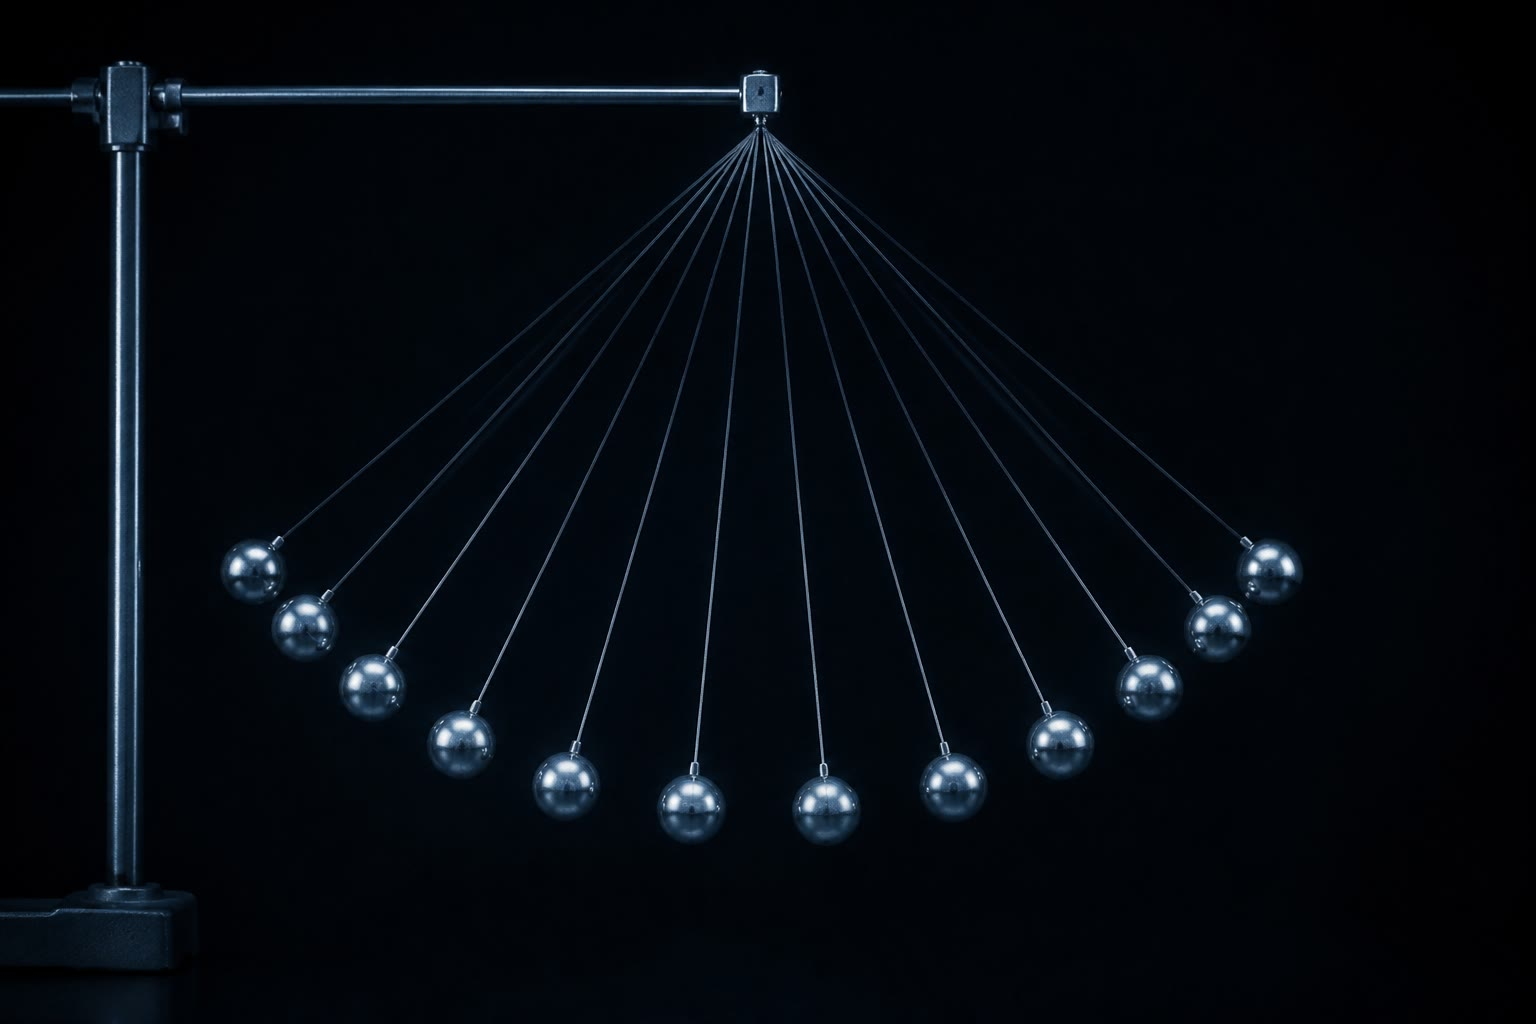
\includegraphics[width=0.58\linewidth]{images/book5/ai/b5-02-pendulum-strobe.jpg}

{\small 频闪下的单摆：摆锤在转折点附近聚集（此处停留较久），在最低点附近分散（此处运动较快）——这是本章用方程描绘的\omterm{def:b3:hamiltonian-mechanics:hamiltonian}{相空间}图像的一张照片。}
\end{omfigure}

\section{练习}

\begin{exercise}[$\star$]\label{exo:b3:hamiltonian-mechanics:1}
对于弹簧上的质量块：(a) 构造 $H$（由 $L$ 出发），并验证 $H =
E_k + E_p$；(b) 写出\omterm{def:b3:hamiltonian-mechanics:hamiltonian}{正则方程}，并验证它们
给出 $\ddot x = -\omega^2x$；(c) 证明轨道在
$(x, p)$ 平面内为椭圆，并给出能量为 $E$ 时的半轴长；
(d) 代表点沿顺时针方向运动，这在什么意义上成立？
\end{exercise}

\begin{exercise}[$\star$]\label{exo:b3:hamiltonian-mechanics:2}
上一章中套在旋转圆环上的珠子，其 $L =
\tfrac12 mR^2\dot\theta^2 + \tfrac12 m\omega^2R^2\sin^2\theta +
mgR\cos\theta$。(a) 计算 $p$ 与 $H$。(b) $H$ 是否守恒？它是否
就是机械能？(c) 对 $H$ 画出等值线草图，分别取
$\omega^2 < g/R$ 与 $\omega^2 > g/R$ 两种情形，并利用该章的有效势能；
(d) 在快速情形下，指出中心、鞍点与
\omterm{def:b3:hamiltonian-mechanics:portrait}{分界线}。
\end{exercise}

\begin{exercise}[$\star$]\label{exo:b3:hamiltonian-mechanics:3}
一个小球在地面上做弹性跳动，$H = p^2/2m + mgz$（$z >
0$）。(a) 画出一次飞行的相轨迹，以及
整个弹跳运动的相轨迹。(b) 弹性碰撞对
代表点有何影响？(c) 计算最大高度为
$z_{\max}$ 时所围的面积，以及\omterm{def:b3:lagrangian-mechanics:action}{作用量} $I$。(d) 玻尔–索末菲规则
$\oint p\,\dd z = nh$ 用于弹跳的中子（$m =
\qty{1.67e-27}{kg}$）时，给出量子化的弹跳高度：估计最低的一个，并与
\qty{15}{\micro m} 作比较，后者是在
2002 年引力量子态实验中测得的。
\end{exercise}

\begin{exercise}[$\star$]\label{exo:b3:hamiltonian-mechanics:4}
仅由正则关系出发，计算 (a) $\{x^2, p\}$；(b)
$\{xp, H\}$，其中 $H = p^2/2m + E_p(x)$，并解释两项的含义
（该括号给出\emph{维里定理}）；(c) $\{L_z, x\}$ 与
$\{L_z, p_x\}$；(d) 证明若 $\{f, H\} = 0$ 且 $\{g, H\} = 0$，
则 $\{f, g\}$ 也守恒（使用雅可比恒等式，在本阶段不加证明地承认：
$\{f,\{g,h\}\} + \{g,\{h,f\}\} + \{h,\{f,g\}\} = 0$）。
\end{exercise}

\begin{exercise}[$\star\star$]\label{exo:b3:hamiltonian-mechanics:5}
单摆靠近其\omterm{def:b3:hamiltonian-mechanics:portrait}{分界线}。(a) 给出\omterm{def:b3:hamiltonian-mechanics:portrait}{分界线}上的能量与
其上的最大 $|p|$。(b) 证明在\omterm{def:b3:hamiltonian-mechanics:portrait}{分界线}上 $p =
\pm 2m\ell^2\omega_0\cos(\theta/2)$，其中 $\omega_0 = \sqrt{g/\ell}$。
(c) 利用 $\dot\theta = p/m\ell^2$，证明从 $\theta$
运动到顶端所需的时间对数发散。(d) 一个刚好在\omterm{def:b3:hamiltonian-mechanics:portrait}{分界线}
下方释放的真实单摆，将在倒立位置附近停留较长
一段时间后才摆回——请将此与 (c) 联系起来，并与
在每个鞍点附近所见的减速现象相联系。
\end{exercise}

\begin{exercise}[$\star\star$]\label{exo:b3:hamiltonian-mechanics:6}
磁场中的带电粒子有 $H = (\vect p -
q\vect A)^2/2m$，其中 $\vect p$ 为上一
章的正则动量。(a) 对 $\vect A = \tfrac12
B(-y, x, 0)$，写出\omterm{def:b3:hamiltonian-mechanics:hamiltonian}{正则方程}并验证其给出回旋运动。(b) 证明 $H =
\tfrac12 m\vect v^{\,2}$：磁场不做功。(c) 计算
两个守恒量 $\pi_x = p_x - \tfrac12
qBy$ 与 $\pi_y = p_y + \tfrac12 qBx$ 的\omterm{def:b3:hamiltonian-mechanics:poisson}{泊松括号}（先验证每个量均守恒），
并证明 $\{\pi_x, \pi_y\} = -qB$：两个守恒量
的括号为常数。(d) 利用
\cref{exo:b3:hamiltonian-mechanics:4}(d)，说明为何
由它们不应再期望得到第三个独立守恒量。
\end{exercise}

\begin{exercise}[$\star\star$]\label{exo:b3:hamiltonian-mechanics:7}
手算验证刘维尔定理。(a) 对自由粒子，流为 $q \to q +
pt/m$，$p \to p$：证明矩形变为
面积相同的平行四边形。(b) 对谐振子，证明流为旋转
（取适当单位）并作出结论。(c) 对\emph{阻尼}振子
$\ddot x = -\omega^2x - \gamma\dot x$，写出流在
$(x, v)$ 平面中的散度，并证明面积按 $\eu^{-\gamma t}$ 缩小：阻尼
不是哈密顿的。(d) 损失的面积在物理上“去”了哪里？
\end{exercise}

\begin{exercise}[$\star\star$]\label{exo:b3:hamiltonian-mechanics:8}
有心势中的平面运动，$H = (p_r^2 + p_\varphi^2/r^2)/2m
+ E_p(r)$。(a) 写出四个\omterm{def:b3:hamiltonian-mechanics:hamiltonian}{正则方程}。(b) 证明 $\{
p_\varphi, H\} = 0$，并指出对应的守恒律。(c) 化为
含有效势能的一维径向\omterm{def:b3:hamiltonian-mechanics:hamiltonian}{哈密顿量}。(d)
对 $E_p = -k/r$，求给定 $p_\varphi$ 时的圆轨道，
并给出其能量——将在
\cref{pb:b3:hamiltonian-mechanics:1}中量子化。
\end{exercise}

\begin{exercise}[$\star\star$]\label{exo:b3:hamiltonian-mechanics:9}
(a) 由正则关系验证 $\{L_x, L_y\} = L_z$。(b)
由轮换推出另外两个\omterm{def:b3:hamiltonian-mechanics:poisson}{泊松括号}。(c) 证明
$\{L^2, L_z\} = 0$。(d) 刚体自由转动，取 $H =
L^2/2J$（球对称转动惯量），证明三个 $L_i$ 均守恒；
若转动惯量互不相等的刚体，结论如何（请
由\omterm{def:b3:hamiltonian-mechanics:poisson}{泊松括号}定性作答）？
\end{exercise}

\begin{exercise}[$\star\star\star$]\label{exo:b3:hamiltonian-mechanics:10}
旧量子论的能级。(a) 证明对谐振子应用 $\oint p\,\dd q = nh$
可得 $E_n = n\hbar\omega$，利用
\cref{prop:b3:hamiltonian-mechanics:sho-action}。(b) 将其用于长为 $a$ 的
一维箱中粒子，并精确恢复 $E_n =
n^2h^2/8ma^2$。(c) 将双原子分子视为劲度系数
为 $k = \qty{1.9e3}{N/m}$、约化质量为 $\qty{1.14e-26}
{kg}$（一氧化碳）的振子，求以 eV 计的 $\hbar\omega$ 及
$n = 1 \to 0$ 发射的波长，并指出它位于
哪一光谱区？(d) 真实能级为 $(n + \tfrac12)\hbar\omega$，那么缺失的
一半是否改变\emph{发射}的波长？哪一实验
能探测零点能的那一半？
\end{exercise}

\begin{exercise}[$\star\star\star$]\label{exo:b3:hamiltonian-mechanics:11}
\omterm{prop:b3:hamiltonian-mechanics:adiabatic}{绝热不变量} $E/\omega$ 的推导。一质量块系于弹簧上，其
劲度系数 $k(t)$ 缓慢增长。(a) 证明沿精确运动 $\dot E = \tfrac12\dot k\,
x^2$。(b) 在 $k$ 固定时对一个周期取平均：
利用 $\langle\tfrac12 kx^2\rangle = E/2$，证明 $\langle\dot E\rangle
= \dot k\,E/2k$。(c) 由此可得 $\dd\ln E = \tfrac12\dd\ln k = \dd\ln
\omega$，从而 $E/\omega$ 为常数。(d) 一单摆以振幅
$\theta_0 = 5^\circ$ 摆动，其摆线被缓慢缩短，自
\qty{1.0}{m}减至\qty{0.5}{m}：求新的振幅及能量增长的
倍数，并说明能量来自何处。
\end{exercise}

\begin{exercise}[$\star\star\star$]\label{exo:b3:hamiltonian-mechanics:12}
单摆\omterm{def:b3:hamiltonian-mechanics:portrait}{分界线}内的面积，恰为一定数目的量子
态的数目。(a) 证明沿\omterm{def:b3:hamiltonian-mechanics:portrait}{分界线}绕行的 $\oint p\,\dd\theta$ 等于
$16m\ell^2\omega_0$。(b) 由玻尔–索末菲条件，能量低于\omterm{def:b3:hamiltonian-mechanics:portrait}{分界线}的量子态数
目为 $N \approx
16m\ell^2\omega_0/h$，计算一克质量悬于
\qty{10}{cm}摆线上的值。(c) 对类氨分子振子求其值，
取 $m \sim \qty{1e-26}{kg}$，$\ell \sim \qty{1e-10}{m}$，
$\omega_0 \sim \qty{1e14}{rad/s}$。(d) 作出结论：需要 $\hbar$ 的力学与
不需要它的力学之间的界限在哪里？
\end{exercise}

\section{问题：旧量子论与氢原子}

\begin{problem}[{周末问题 --- 量子化相空间，
估算里德伯常量}]\label{pb:b3:hamiltonian-mechanics:1}
1913 年玻尔以行星力学
加一条量子规则计算了氢原子光谱；索末菲将该规则认作
关于\omterm{def:b3:hamiltonian-mechanics:hamiltonian}{相空间}面积的一种表述。本题用本章的工具重建他们的
计算。数据：$m_{\text{e}} =
\qty{9.11e-31}{kg}$，$e = \qty{1.60e-19}{C}$，$1/4\pi\varepsilon_0 =
\qty{8.99e9}{N.m^2/C^2}$，$h = \qty{6.63e-34}{J.s}$，$c =
\qty{3.00e8}{m/s}$。记 $k = e^2/4\pi\varepsilon_0$。

\medskip\noindent\textbf{第一部分 --- 开普勒\omterm{def:b3:hamiltonian-mechanics:hamiltonian}{哈密顿量}。}
一个电子在平面内绕固定质子运动。
\begin{enumerate}
  \item 说明将质子视为固定的依据（质量比），并写出
        \omterm{def:b3:hamiltonian-mechanics:hamiltonian}{哈密顿量} $H = \dfrac{p_r^2}{2m_{\text{e}}} +
        \dfrac{p_\varphi^2}{2m_{\text{e}}r^2} - \dfrac{k}{r}$。
  \item 写出四个\omterm{def:b3:hamiltonian-mechanics:hamiltonian}{正则方程}。
  \item 证明 $p_\varphi$ 守恒，并指出其名称。
  \item 将径向运动归结为有效势能
        $U_{\text{有效}}(r) = p_\varphi^2/2m_{\text{e}}r^2 - k/r$，并
        画出其草图。
  \item 求圆轨道：$r_{\text{c}} =
        p_\varphi^2/m_{\text{e}}k$。
  \item 证明其能量为 $E = -k/2r_{\text{c}} =
        -m_{\text{e}}k^2/2p_\varphi^2$，并验证它是势能的
        一半（本科一年级分册中的
        引力轨道的维里比）。
\end{enumerate}

\medskip\noindent\textbf{第二部分 --- 经典轨道。}
\begin{enumerate}[resume]
  \item 对半径为 $r$ 的圆轨道，求速率 $v$ 与
        轨道频率 $f_{\text{轨道}}$ 作为 $r$ 的函数。
  \item 一条原子尺度的轨道，$r = \qty{0.05}{nm}$：计算 $v$
        （以及 $v/c$）、$f_{\text{轨道}}$，并求以 eV 为单位的能量。
  \item 计算该轨道的角动量 $p_\varphi$，
        并将其与 $\hbar = h/2\pi$ 比较：这种接近
        说明了什么？
  \item 经典地看，绕核运动的电子是一个振荡偶极子，
        以 $f_{\text{轨道}}$ 辐射电磁波（见本科二年级分册）；其能量
        约在 \qty{1e-11}{s} 内衰减。指出这一图像对原子所作的两个
        致命预言，并说明实际观测到的
        是什么。
  \item 观测到的光谱具有哪一特征（分立谱线、
        组合规则 $1/\lambda = R_H(1/n^2 - 1/n'^2)$），从而启示了
        分立的能量\emph{能级}？
  \item 解释为何\emph{\omterm{prop:b3:hamiltonian-mechanics:adiabatic}{绝热不变量}}是
        取固定普适值之量的自然候选
        （回顾\cref{prop:b3:hamiltonian-mechanics:adiabatic}）。
\end{enumerate}

\medskip\noindent\textbf{第三部分 --- 量子化。}
对圆轨道的角向运动施加索末菲法则：
$\oint p_\varphi\,\dd\varphi = nh$, $n = 1, 2, 3, \dots$
\begin{enumerate}[resume]
  \item 证明该法则可写为 $p_\varphi = n\hbar$。
  \item 推出允许半径 $r_n = n^2a_0$，其中 $a_0 =
        \hbar^2/m_{\text{e}}k$，并计算 $a_0$。
  \item 推出允许能量 $E_n = -E_{\text{I}}/n^2$，其中
        $E_{\text{I}} = m_{\text{e}}k^2/2\hbar^2$，并计算
        $E_{\text{I}}$ 以焦耳和 eV 为单位。
  \item 计算第一轨道上的速率，并验证 $v_1/c =
        k/\hbar c \approx 1/137$（精细结构常数）。
  \item 一个光子携带跃迁的能量：推导
        里德伯公式以及 $R_H = E_{\text{I}}/hc$ 的值；
        与实测值 \qty{1.097e7}{m^{-1}} 比较。
  \item 计算跃迁 $2 \to 1$、
        $3 \to 2$ 与 $\infty \to 2$ 的波长；其中哪一条可见，呈何种
        颜色？
  \item 电离氦离子 He$^+$ 即核电荷为 $2e$ 的氢原子：
        $a_0$ 与 $E_{\text{I}}$ 如何标度，其 $2 \to 1$ 谱线
        落在何处？
\end{enumerate}

\medskip\noindent\textbf{第四部分 --- 对照。}
\begin{enumerate}[resume]
  \item 计算轨道频率 $f_{\text{轨道}}(n)$ 与
        跃迁频率 $\nu_{n \to n-1}$，取 $n = 2$、$10$、
        $100$，并证明其比值趋于 $1$（随 $n$ 增大）。
  \item 这就是玻尔的\emph{对应原理}：用
        一句话陈述之。
  \item 法则 $p_\varphi = n\hbar$ 从 $n = 1$ 开始：若取 $n = 0$，
        对圆轨道而言将意味着什么荒谬之处？
  \item 量子力学将严格保留 $E_n = -E_{\text{I}}/n^2$，
        却舍弃了轨道图像。试举出轨道图像所错误预言的两个可测
        事实（基态角动量的
        大小；具有相同 $n$ 而形状不同的态的存在
        性）。
  \item μ子是质量为电子 $207$ 倍的“重电子”：对于μ子
        氢原子，计算 $a_0^\mu$ 与 $E_{\text{I}}^\mu$，并
        解释为何μ子原子能够探测\emph{原子核}。
  \item 概述这一著名结果：一个\omterm{prop:b3:hamiltonian-mechanics:adiabatic}{绝热不变量}取为
        $h$ 的整数倍，便得到 $a_0 = \qty{52.9}{pm}$，
        $E_{\text{I}} = \qty{13.6}{eV}$，以及
        四位有效数字的氢光谱 --- 并为真正的理论提供它的两个
        核心常量。
\end{enumerate}
\end{problem}
